\begin{frame}{Intro to Lagrangian Floats}
     \centering
     \includegraphics[height=0.7\textheight,width=0.7\textwidth,keepaspectratio]{images/VOLT/m-aue-swarm-render.png}
     \includegraphics[height=0.7\textheight,width=0.7\textwidth,keepaspectratio]{images/VOLT/volt-m-aue-swarm.png}
\end{frame}

\begin{frame}{Components of VOLT}
     \centering
     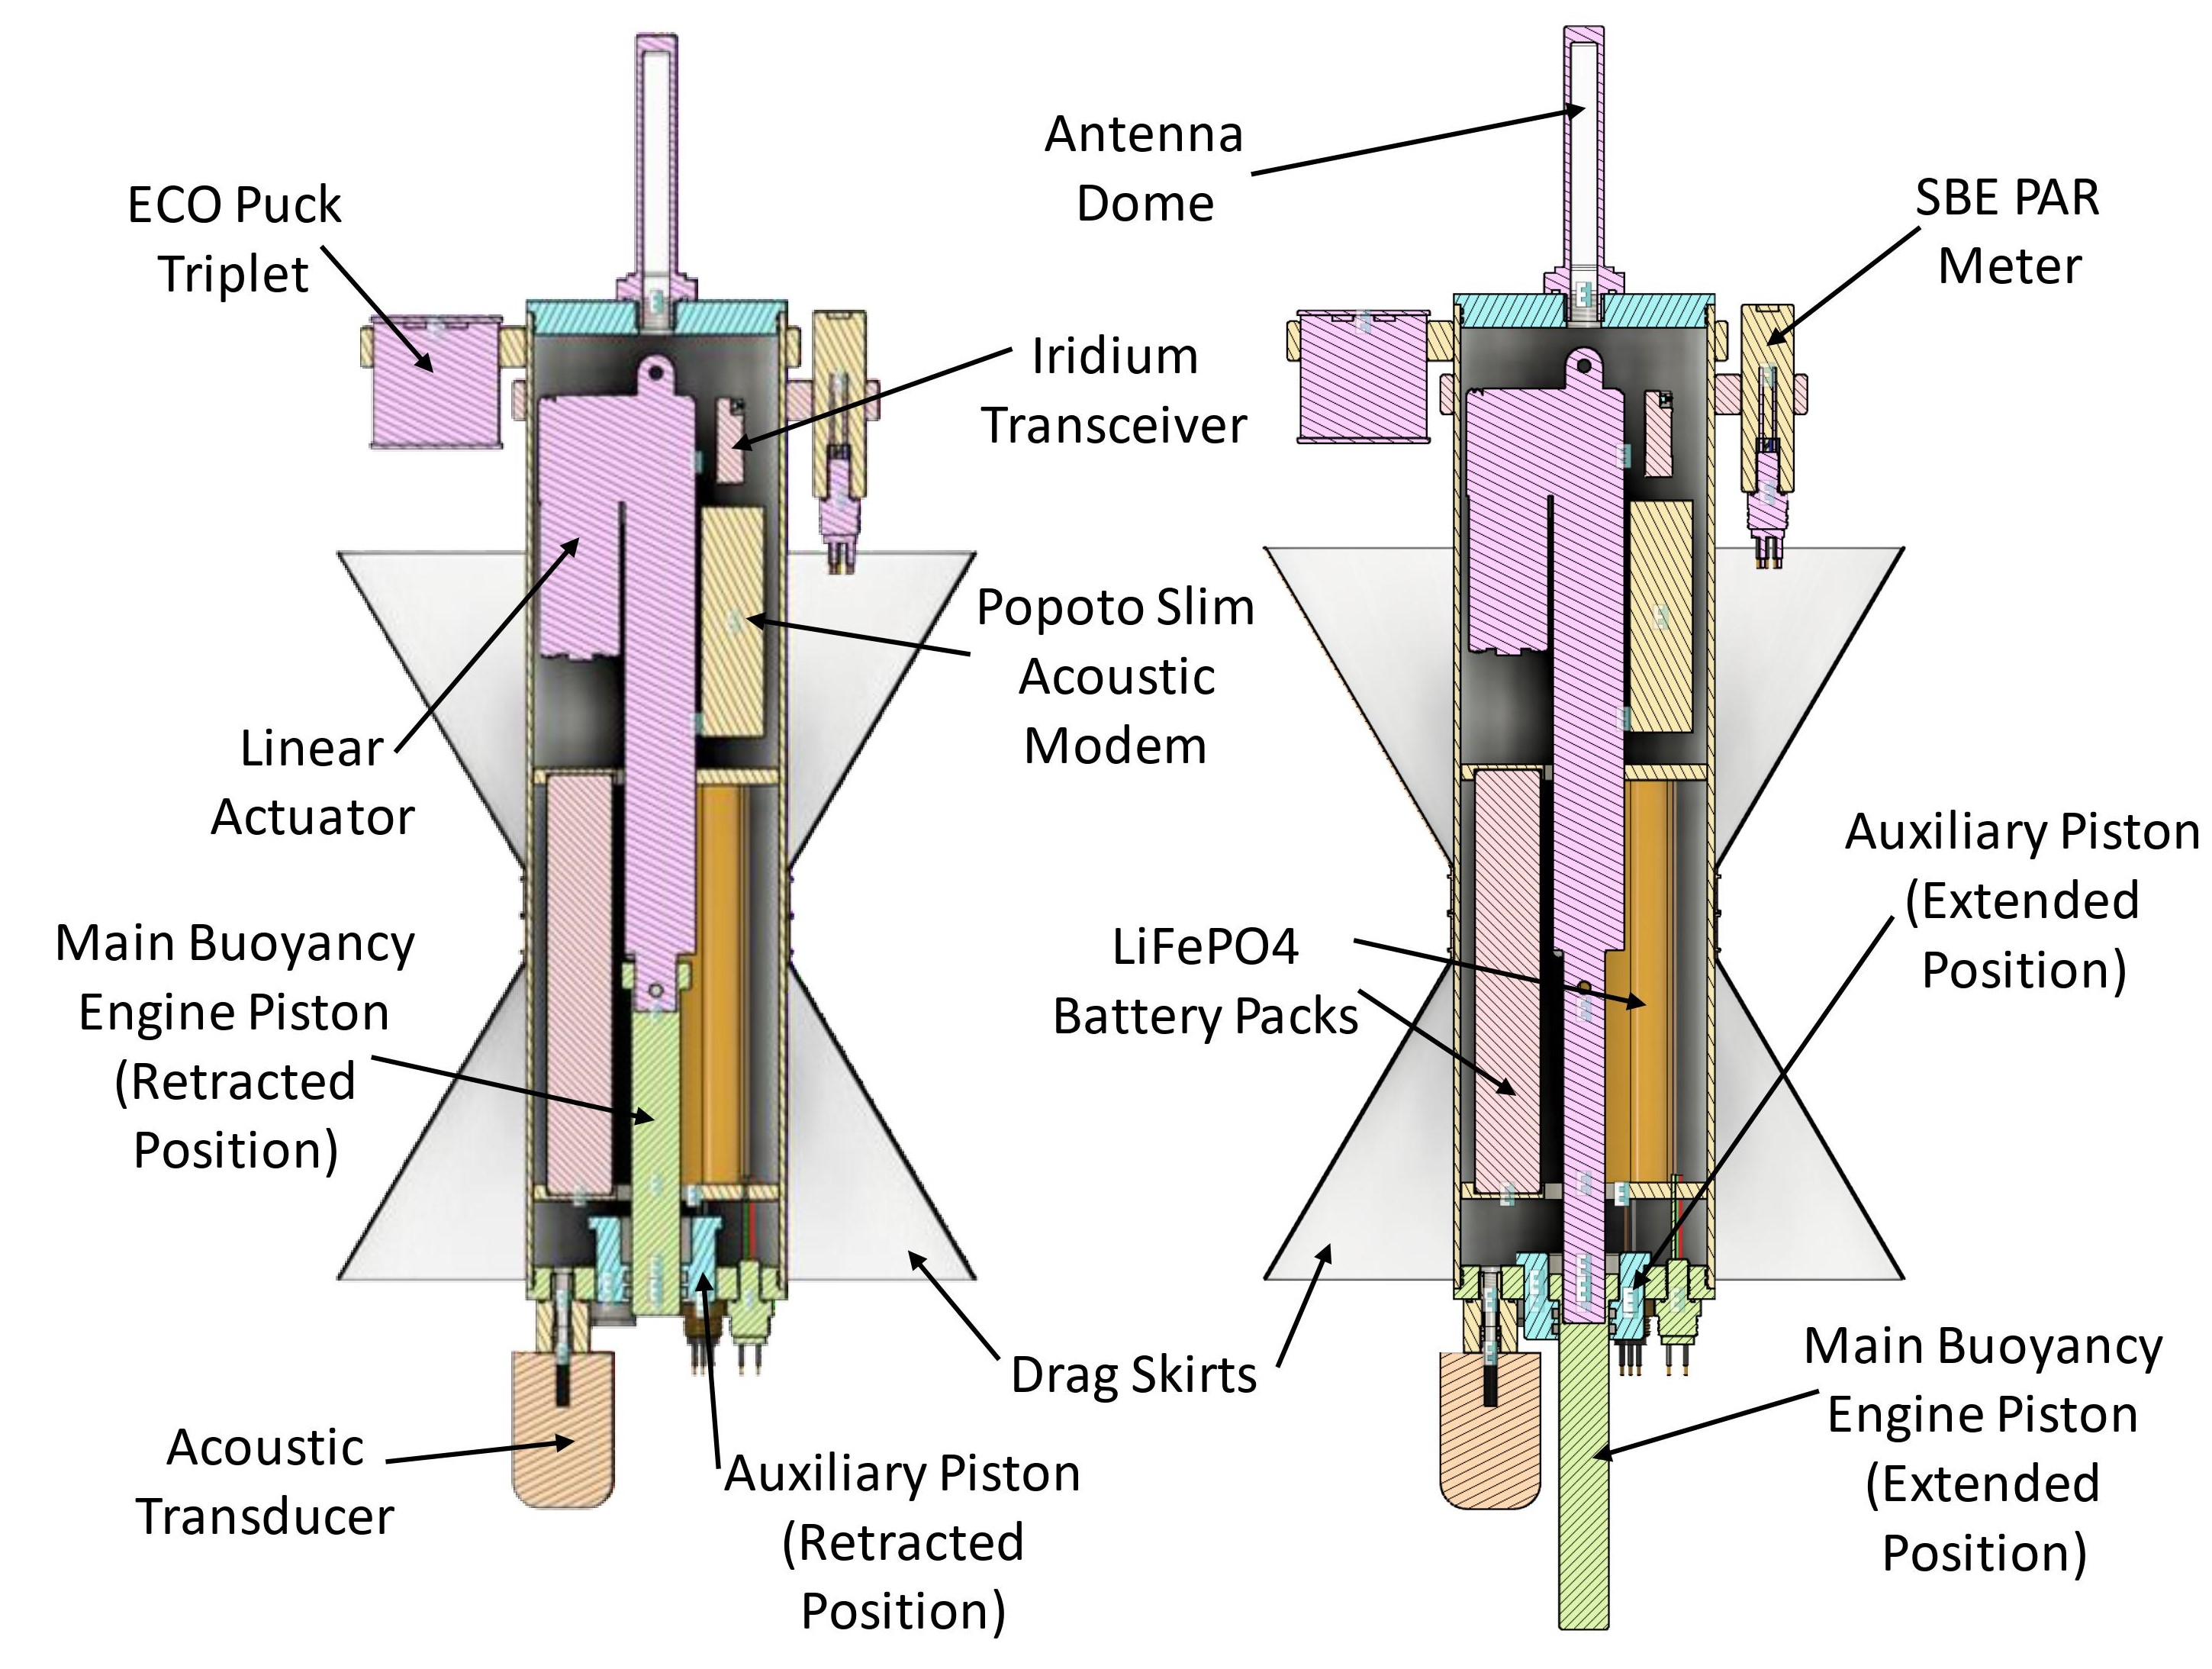
\includegraphics[height=0.8\textheight,width=0.8\textwidth,keepaspectratio]{images/VOLT/volt-sectionview.png}
     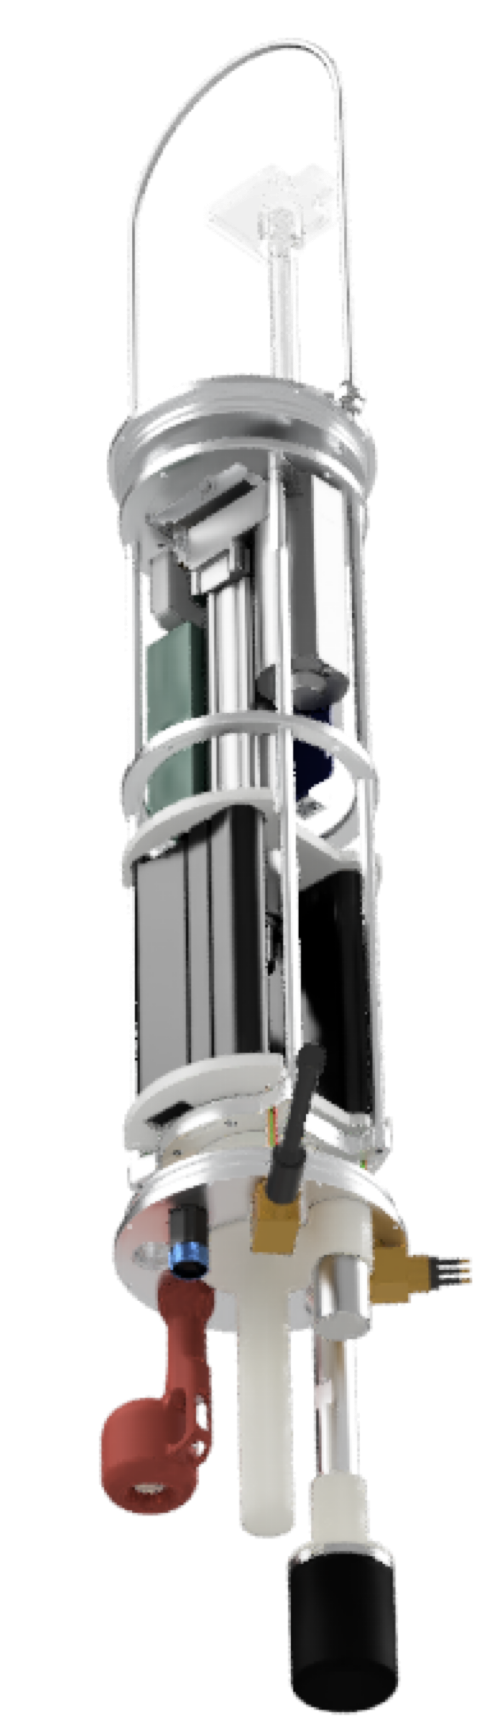
\includegraphics[height=0.9\textheight,width=0.9\textwidth,keepaspectratio]{images/VOLT/volt-rendered.png}
\end{frame}

\begin{frame}{My Work So Far: Battery PCB}
    \centering
    \includegraphics[height=0.5\textheight,width=0.5\textwidth,keepaspectratio]{images/VOLT/batterypcbschematic.png}
    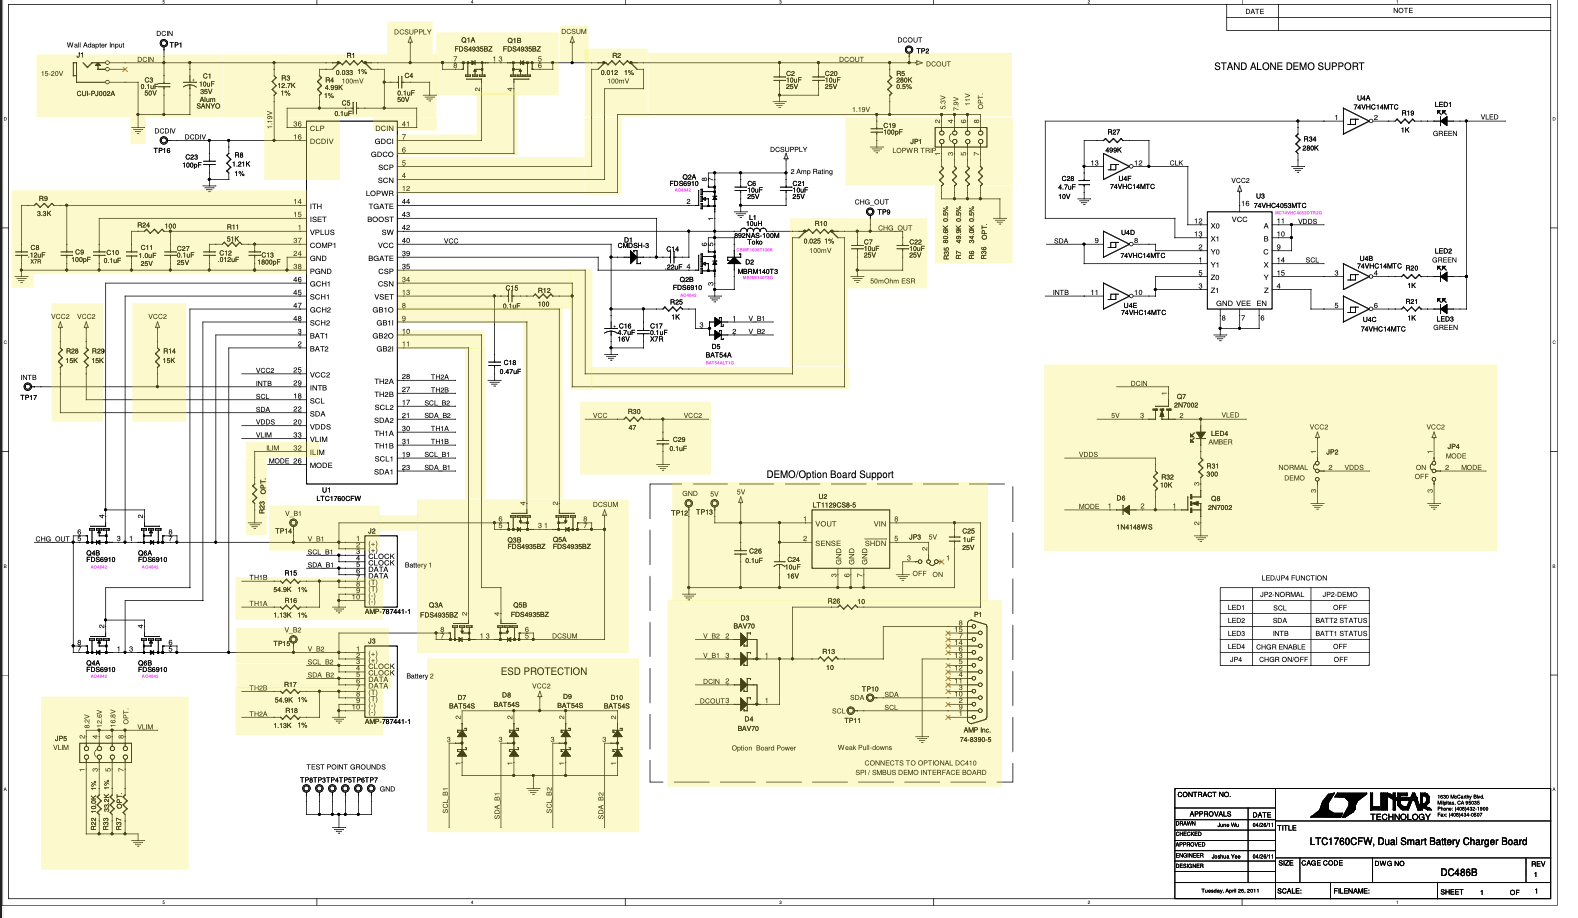
\includegraphics[height=0.5\textheight,width=0.5\textwidth,keepaspectratio]{images/VOLT/demo-board-schematic.png}
\end{frame}

\begin{frame}{Future/In-Progress Work: Localization}
    \centering
    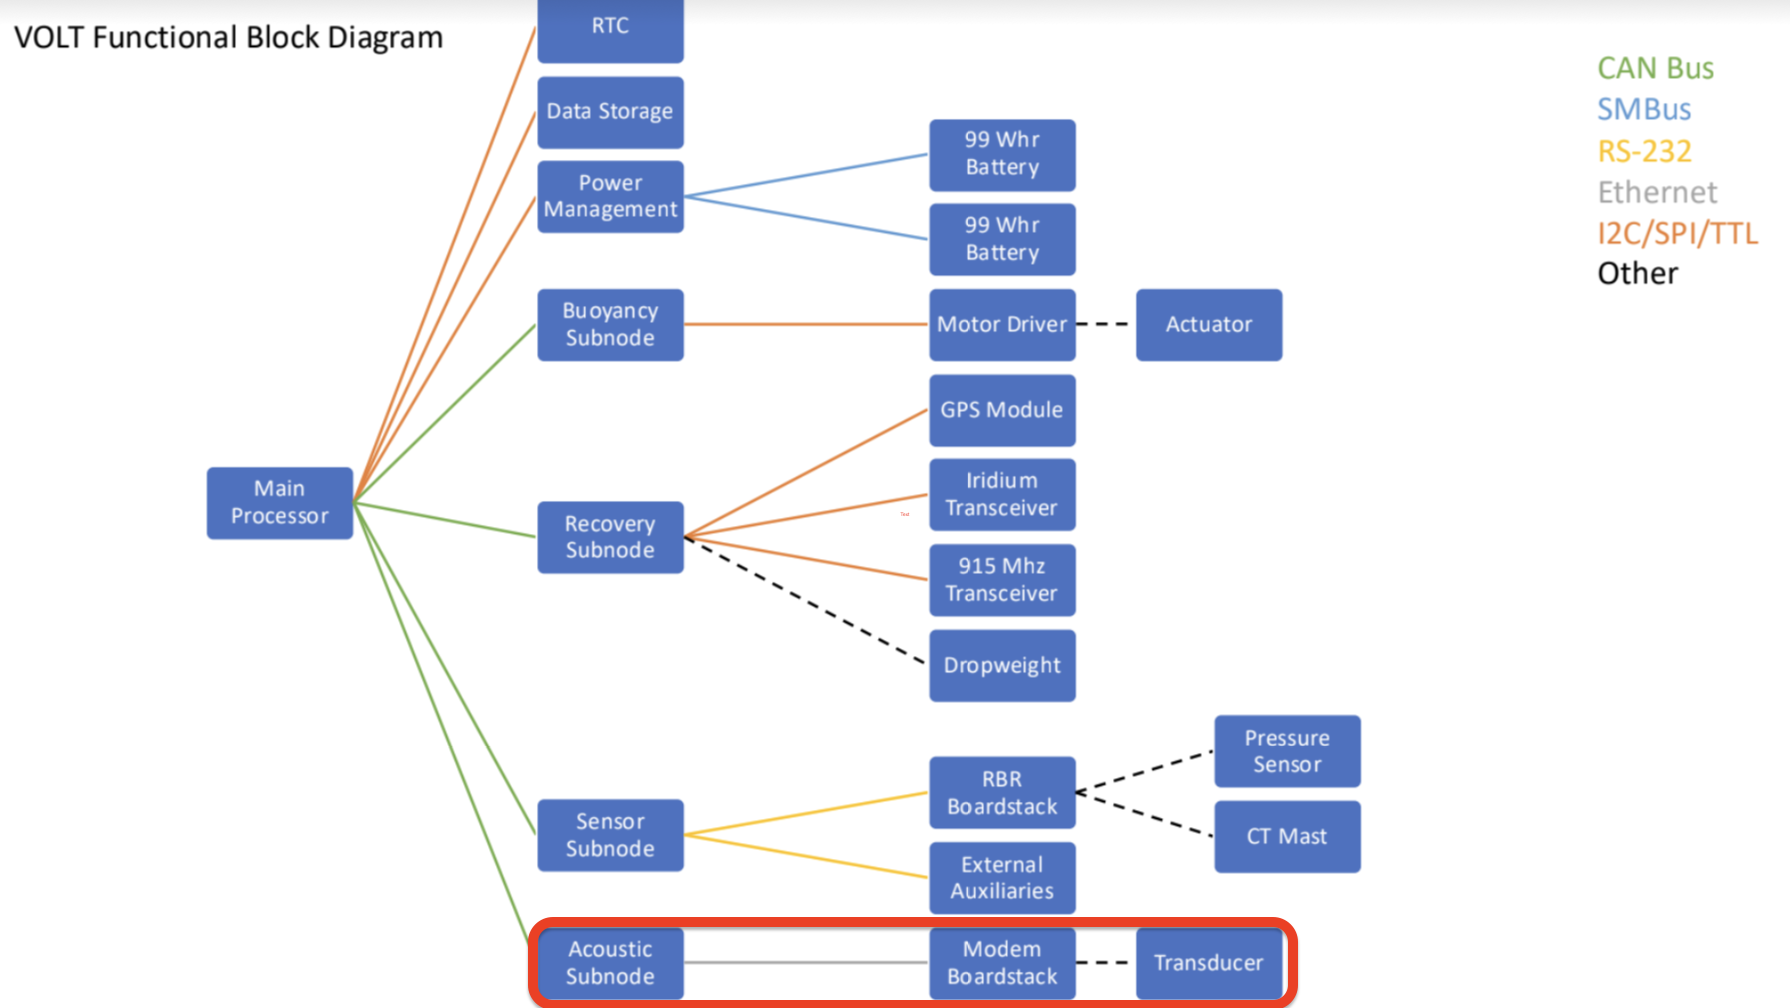
\includegraphics[height=0.8\textheight,width=0.8\textwidth,keepaspectratio]{images/VOLT/volt-blockdiagram.png}
\end{frame}
    

% To create a slide with a bullet list, use the following:
% \begin{frame}{TITLE}
%     \begin{itemize}
%         \item ITEM 1
%         \item ITEM 2
%     \end{itemize}    
% \end{frame}

% To create a slide with numbered list, use the following:
% \begin{frame}{TITLE}
%     \begin{enumerate}
%         \item ITEM 1
%         \item ITEM 2
%     \end{enumerate}
% \end{frame}

% To create a slide with a graphic:
% 1. Add the graphic to this folder (named picture.png)
% 2. Use the following:
% \begin{frame}{TITLE}
%     \centering
%     \includegraphics[height=0.7\textheight,width=0.7\textwidth,keepaspectratio]{picture.png}
% \end{frame}

% To create a slide with two columns, use the following:
% \begin{frame}{TITLE}
%     \begin{columns}
%         \begin{column}{0.5\textwidth}
%             COLUMN 1 BODY
%         \end{column}
%         \begin{column}{0.5\textwidth}
%             COLUMN 2 BODY
%         \end{column}
%     \end{columns}
% \end{frame}
